\chapter{Marco Metodológico}

En este capítulo se enuncian las directrices para la implementación
del presente Proyecto de Grado, la Figura \ref{fig:metodo} refleja la metodología empleada.
En primer lugar, en la Sección \ref{sec:MedRecDat},
se detallan los pasos a seguir para la recopilación de los datos en \textit{PostgreSQL}.
Posteriormente, en la Sección \ref{sec:MedProcCod}, se explica cómo se procesan los fragmentos 
de código para la creación de la firma y la elaboración del índice invertido. 
Finalmente, en la Sección \ref{sec:MedConSisRec}, se proveen los lineamientos para la
creación del Sistema de Recomendación.

\begin{figure}[h]
\centering
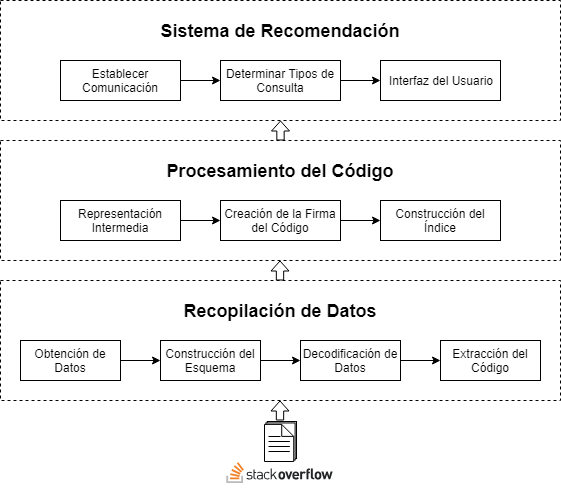
\includegraphics[width=30em]{img/metodo.png}
\caption{Esquema de Metodológico}
\label{fig:metodo}
\end{figure}

\section{Recopilación de Datos}
\label{sec:MedRecDat}

La información utilizada proviene de la base de
datos de \textit{Stack Overflow} del año $2014$,
es publicada en el formato \ac{XML} y
obtenida mediante el protocolo de transferencia \textit{BitTorrent}.
Además, es provista de forma libre bajo la licencia \textit{cc-by-sa 3.0},
que permite compartir y adaptar el contenido
si se atribuye el crédito a sus autores originales.

A continuación, se extraen los archivos de la base de datos y
la información es recopilada en \textit{PostgreSQL} para su posterior uso.

\subsection{Obtención de Datos}

Se obtienen y extraen los archivos \ac{XML} pertenecientes
a la base de datos de \textit{Stack Overflow},
los cuales se encuentran comprimidos en el formato \textit{7z},
utilizando la compresión \textit{bzip2}.
Una descripción detallada del contenido de los archivos 
se da en la Sección \ref{subsec:EstBasDat}.

\subsection{Construcción del Esquema}

Cada archivo \ac{XML} representa una tabla en la base de datos, 
donde los elementos bajo la etiqueta \textit{row} representan 
las filas y sus atributos representan las columnas.
Por este motivo, se utiliza \textit{PostgreSQL} para recopilar los datos,
ya que provee un conjunto de funciones para manipular texto en el formato \ac{XML}.

Estas funciones se emplean para desarrollar una serie de \textit{scripts}
en el lenguaje \ac{PL/pgSQL}, que permiten reproducir el esquema de
la base de datos de \textit{Stack Overflow}.

\subsection{Decodificación de Datos}

Los datos contienen entidades especiales en el formato \ac{XML}
que deben ser decodificadas para darle sentido a los tópicos.
Algunos de estas son: \lstinline{&amp;}, \lstinline{&lt;}, \lstinline{&gt;}.

Es de notar que la función \lstinline{xpath()} perteneciente a \textit{PostgreSQL},
es capaz de decodificar las entidades \ac{XML} al extraer los atributos de los elementos,
siempre que la versión de \textit{PostgreSQL} sea previa a la \textit{v9.2}~\cite{CAAY5AM3Cj}.

\subsection{Extracción del Código}

Un tópico %, ya sea éste una pregunta o una respuesta,
puede contener varios fragmentos de código dentro del cuerpo,
que se encuentra en formato \ac{HTML}.
Para extraer estos fragmentos,
se separa el texto contenido dentro de la etiqueta \lstinline{<code>}
y se almacena en una tabla independiente. 

Sin embargo, solo se consideran aquellos fragmentos de código que,
adicionalmente, se encuentran dentro de la etiqueta \lstinline{<pre>};
debido a que, dicha etiqueta es utilizada para mantener
el formato del texto, incluso si éste posee saltos de línea.

\section{Procesamiento del Código}
\label{sec:MedProcCod}

Los fragmentos de código extraídos son transformados en un conjunto de
\textit{n-grams}, lo que permite realizar comparaciones. Luego, 
a partir de esta representación se genera una firma,
que es mucho más compacta y eficiente.

\subsection{Representación Intermedia}
\label{subsec:MedRepInt}

Se emplea un \textit{lexer} para ignorar las modificaciones
de código de Tipo II, mencionados en la Sección \ref{subsec:plagio}.
De esta manera, se identifican los lexemas pertenecientes a los lenguaje c y c++ contenidos en 
el fragmento de código y se genera una secuencia de \textit{tokens}.

Luego, se utiliza la técnica de \textit{n-gram} para transformar la secuencia
de \textit{tokens}, en una representación intermedia que permite evaluar 
la similitud de dos fragmentos de código arbitrario mediante el coeficiente
de similitud de \textit{Jaccard}.

Finalmente, se utiliza una función de \textit{hash} para transformar los
\textit{n-grams} a enteros, permitiendo una representación más compacta
y una comparación más rápida.

\subsection{Creación de la Firma del Código}
\label{subsec:MedFirCod}

Se establece el tamaño de la firma y se calculan las funciones de \textit{hash}
asociadas. Luego, se genera la firma a partir del conjunto de \textit{n-grams}
utilizando el \textit{MinHash}, se almacena y se asocia al fragmento de código
correspondiente.% Dicha técnica, permite estimar el porcentaje de similitud,
%lo que evita operaciones costosas sobre conjuntos.

\subsection{Contrucción de un Índice}
\label{subsec:MedConInd}

Se establece la cantidad de bandas y su tamaño.
Luego, se separa cada firma en minifirmas,
usando la técnica de \ac{LSH}.
Entonces, se crea un índice invertido que almacena
las minifirmas en sus respectivas bandas
y las asocia al fragmento de código correspondiente.

Se puede abordar la creación de un índice invertido que
dependa de un entero si se utiliza una función de \textit{hash}
sobre los elementos de la minifirma.
Sin embargo, \textit{PostgreSQL} permite almacenar arreglos
de tamaño arbitrario y definir sus índices.

\section{Sistema de Recomendación}
\label{sec:MedConSisRec}

La elaboración del Sistema de Recomendación requiere establecer una estructura
de comunicación, determinar los tipos de consulta que se proveen y desarrollar
la interfaz gráfica.

\subsection{Establecer Comunicación}

Se calcula la firma del fragmento de código provisto por el usuario, 
siguiendo los pasos establecidos en las secciones:
Sección \ref{subsec:MedRepInt} y Sección \ref{subsec:MedFirCod}.
Luego, se construye la consulta y se envía al servidor de
bases de datos. El cual recibe la consulta y utiliza el
índice invertido desarrollado en la Sección \ref{subsec:MedConInd}
para retornar una lista de sugerencias.

\subsection{Determinar Tipos de Consulta}

Las consultas realizas por el \textit{Sistema de Recomendación} pueden
ser modificadas, permitiendo un mayor control sobre las 
sugerencias realizadas.

Las posibles modificaciones incluyen filtros que permitan
limitar las sugerencias, así como refinar la búsqueda
mediante el uso de distintas categorías.
Adicionalmente, se puede cambiar el orden por defecto,
ordenando los tópicos por reputación.

\subsection{Interfaz del Usuario}

El Sistema de Recomendación se provee con una interfaz
sencilla, que se compone de tres elementos.
Un botón de uso que permite capturar el fragmento de código
resaltado por el usuario, una ventana para
configurar las opciones de búsqueda y una 
ventana para mostrar las sugerencias.